\section{MapReduce Service}\label{mapreduce_service}
This section will explore logical the design of the MapReduce operation performed as a Grid Service. The process is modeled using three Petri Nets, each one providing the point of view of one among the possible involved entities types: Map Worker, Reduce Worker and MapReduce Master.

Every Petri Net that will be presented assumes that the Resources' retrieval process (viewed in \textit{figure \ref{fig:use_cases_satisfaction_node_contribution}}) has already been performed, allowing to focus on the actual MapReduce process itself.
Furthermore, in every Petri Net snapshot provided, transitions that can be transitioned (in that particular configuration of the places) are highlighted in red to facilitate its understanding.
  
\subsection{Map Worker}
TODO

\begin{figure}[!ht]
    \centering
    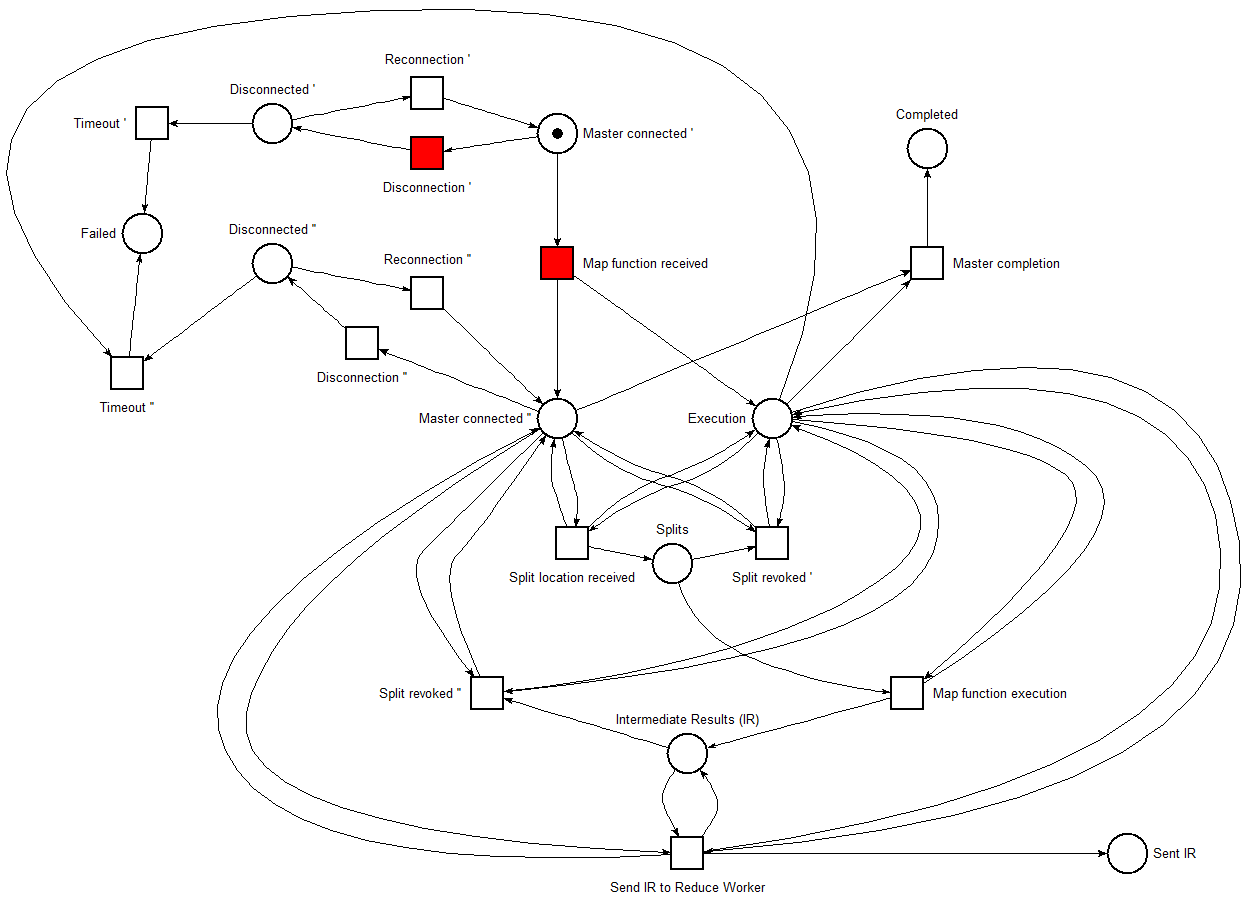
\includegraphics[width=\linewidth]{document/chapters/chapter_6/images/map_worker_petri_net_1.png}
    \caption{Map Worker - Start}
    \label{fig:map_worker_petri_net_1}
\end{figure}

\begin{figure}[!ht]
    \centering
    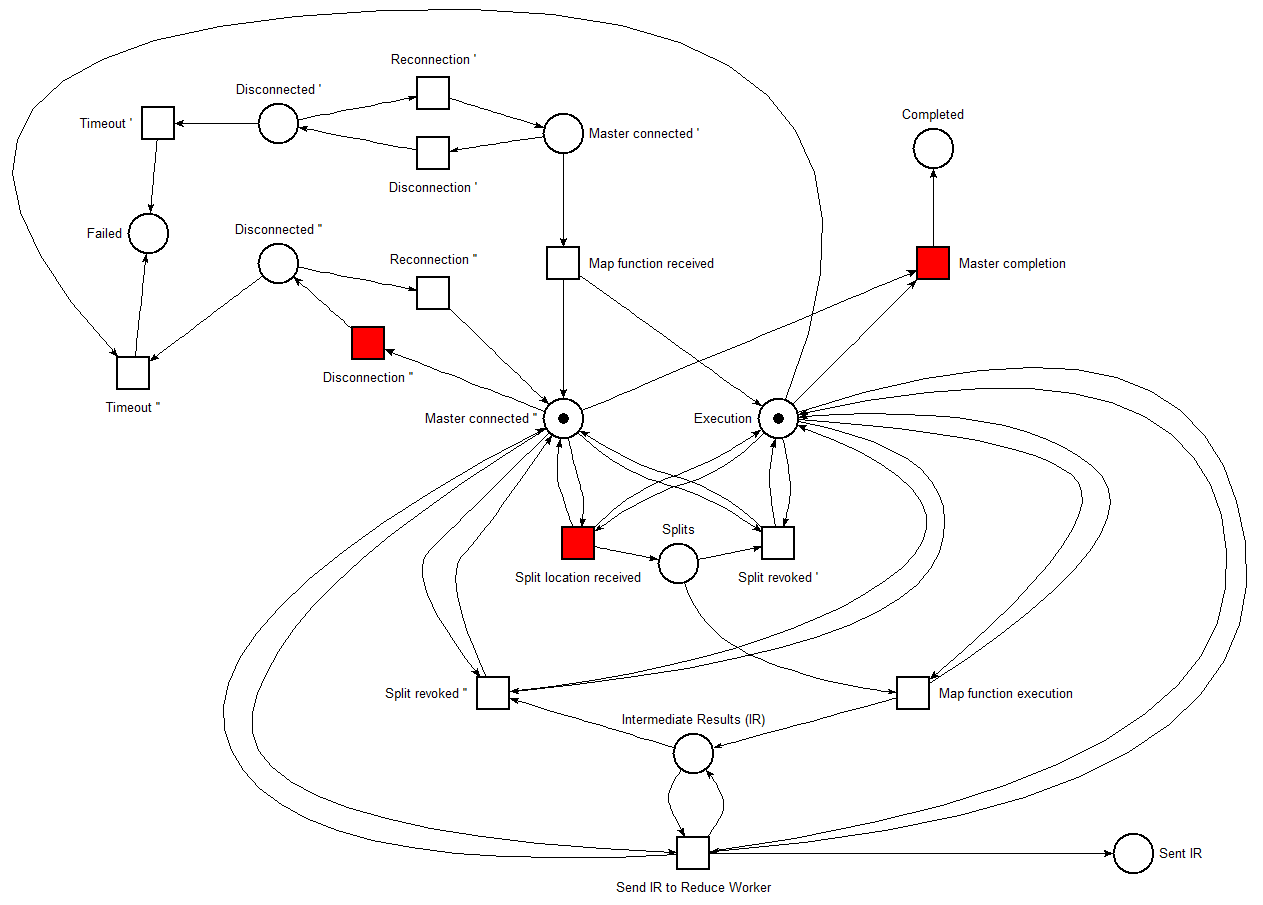
\includegraphics[width=\linewidth]{document/chapters/chapter_6/images/map_worker_petri_net_2.png}
    \caption{Map Worker - Mapping}
    \label{fig:map_worker_petri_net_2}
\end{figure}

\begin{figure}[!ht]
    \centering
    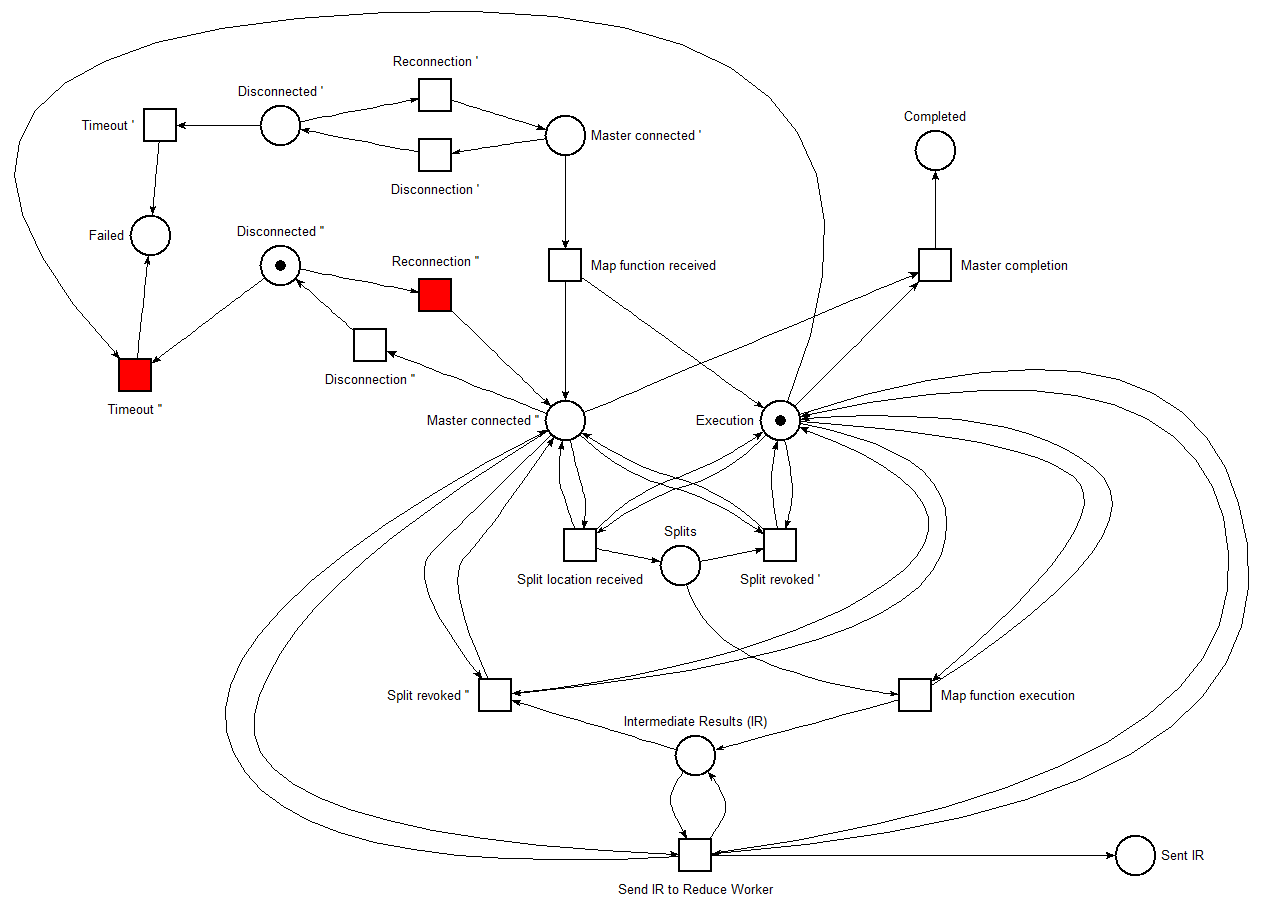
\includegraphics[width=\linewidth]{document/chapters/chapter_6/images/map_worker_petri_net_3.png}
    \caption{Map Worker - Intermediate Result sent}
    \label{fig:map_worker_petri_net_3}
\end{figure}

\begin{figure}[!ht]
    \centering
    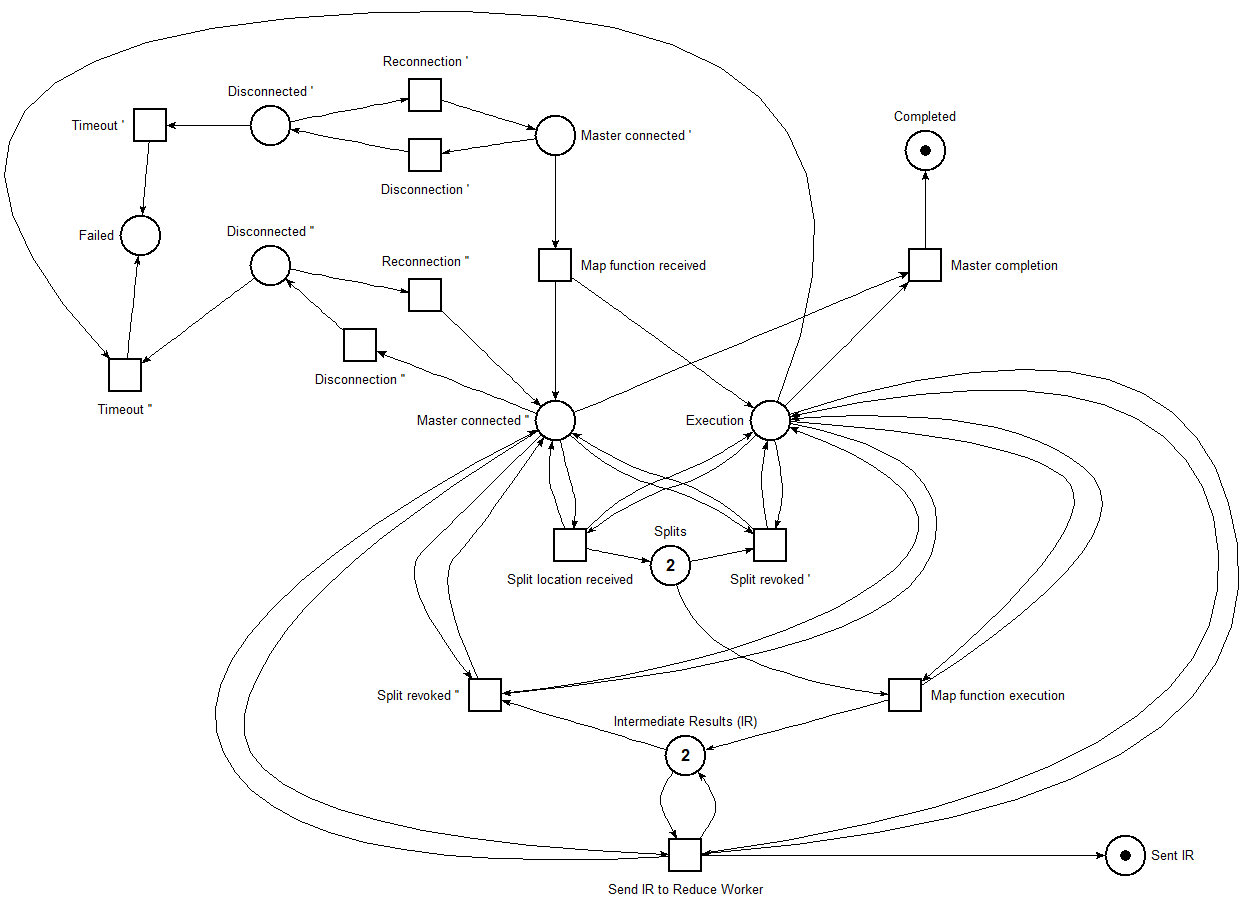
\includegraphics[width=\linewidth]{document/chapters/chapter_6/images/map_worker_petri_net_4.png}
    \caption{Map Worker - Completion}
    \label{fig:map_worker_petri_net_4}
\end{figure}

\subsection{Reduce Worker}
TODO

\begin{figure}[!ht]
    \centering
    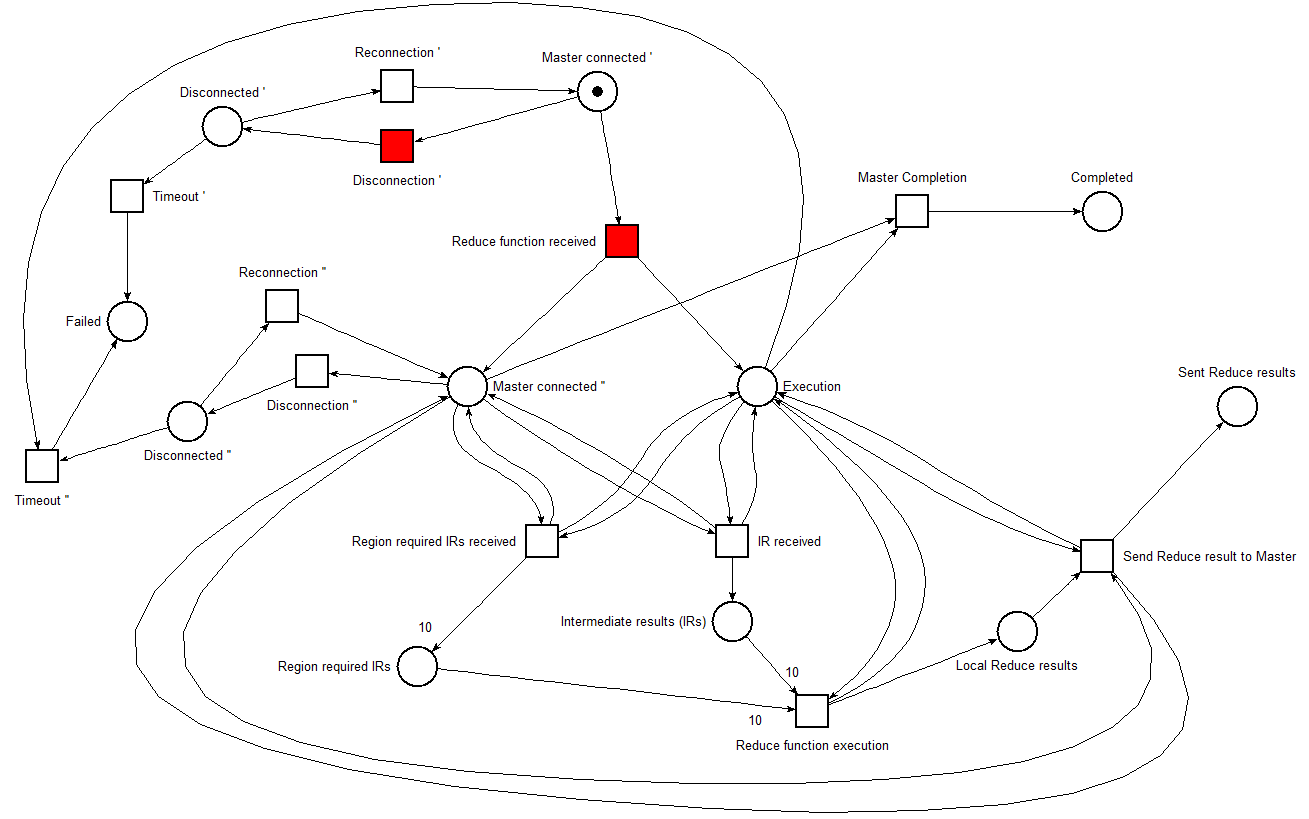
\includegraphics[width=\linewidth]{document/chapters/chapter_6/images/reduce_worker_petri_net_1.png}
    \caption{Reduce Worker - Local result}
    \label{fig:map_worker_petri_net_1}
\end{figure}

\begin{figure}[!ht]
    \centering
    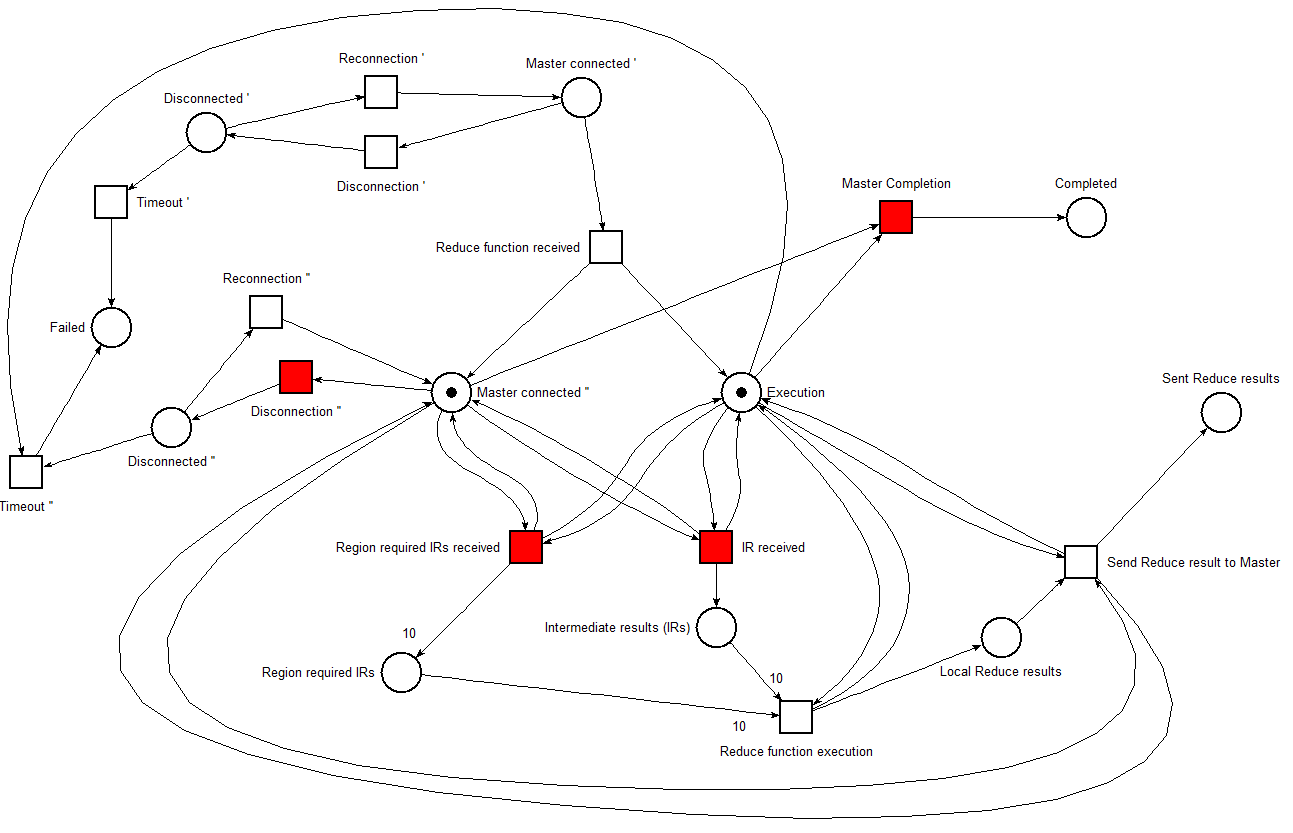
\includegraphics[width=\linewidth]{document/chapters/chapter_6/images/reduce_worker_petri_net_2.png}
    \caption{Reduce Worker - Completion}
    \label{fig:map_worker_petri_net_2}
\end{figure}

\subsection{MapReduce Master}
TODO

\begin{figure}[!ht]
    \centering
    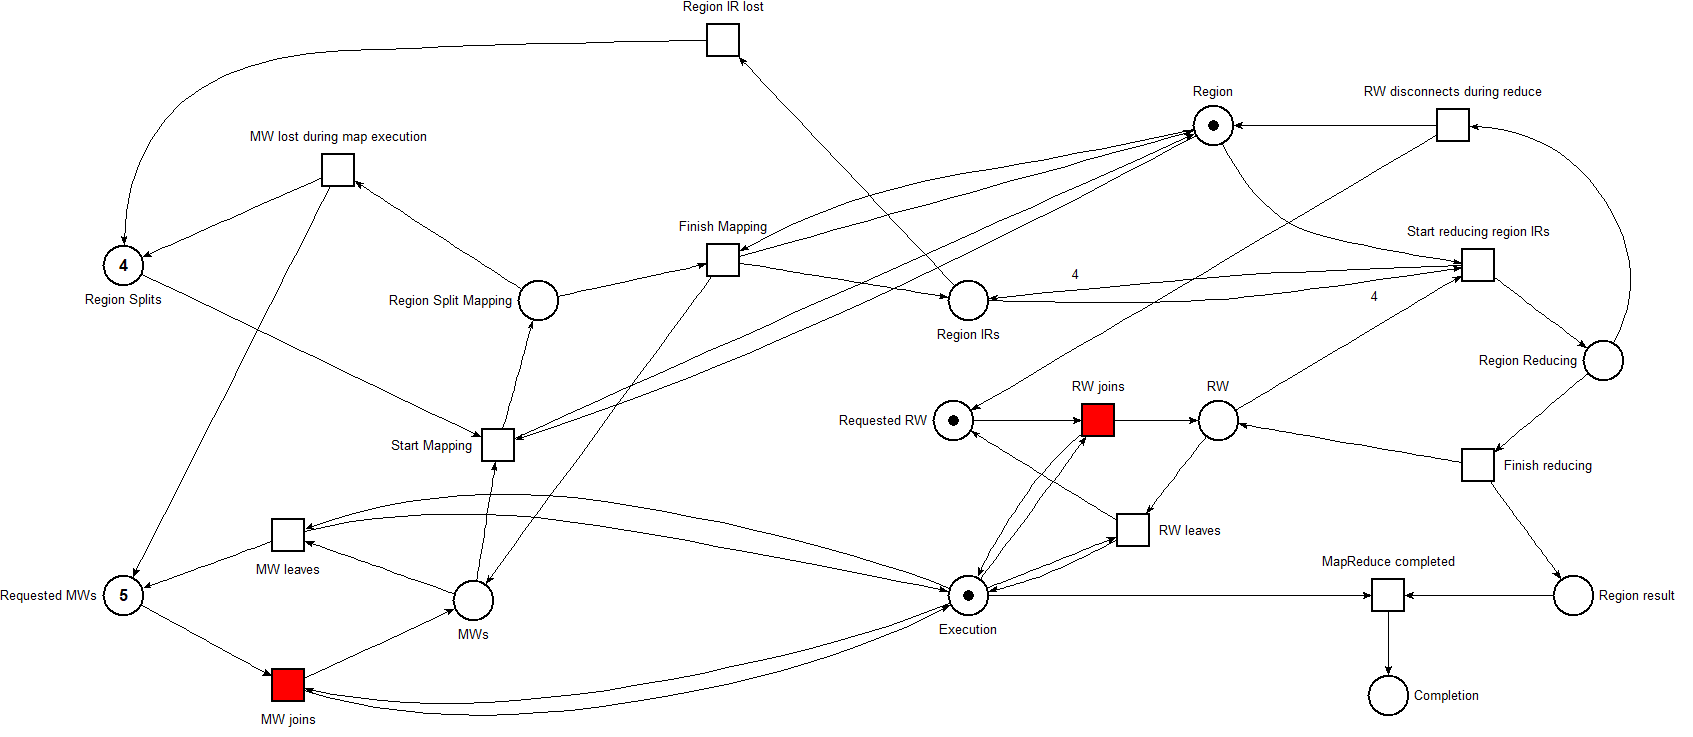
\includegraphics[width=\linewidth]{document/chapters/chapter_6/images/master_petri_net_1.png}
    \caption{MapReduce Master - Recruitment}
    \label{fig:master_petri_net_1}
\end{figure}

\begin{figure}[!ht]
    \centering
    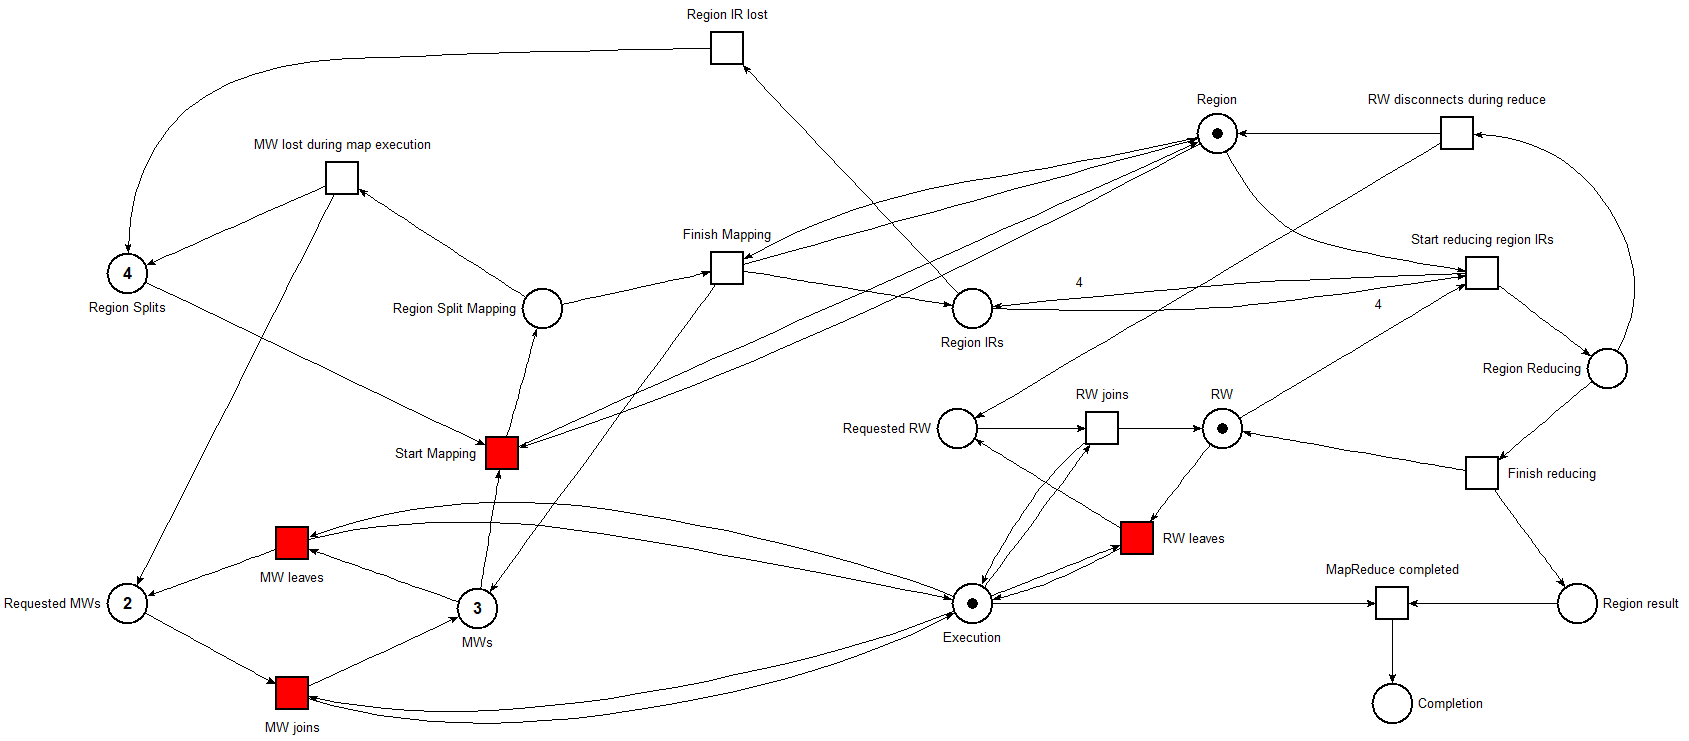
\includegraphics[width=\linewidth]{document/chapters/chapter_6/images/master_petri_net_2.png}
    \caption{MapReduce Master - Mapping process}
    \label{fig:master_petri_net_2}
\end{figure}

\begin{figure}[!ht]
    \centering
    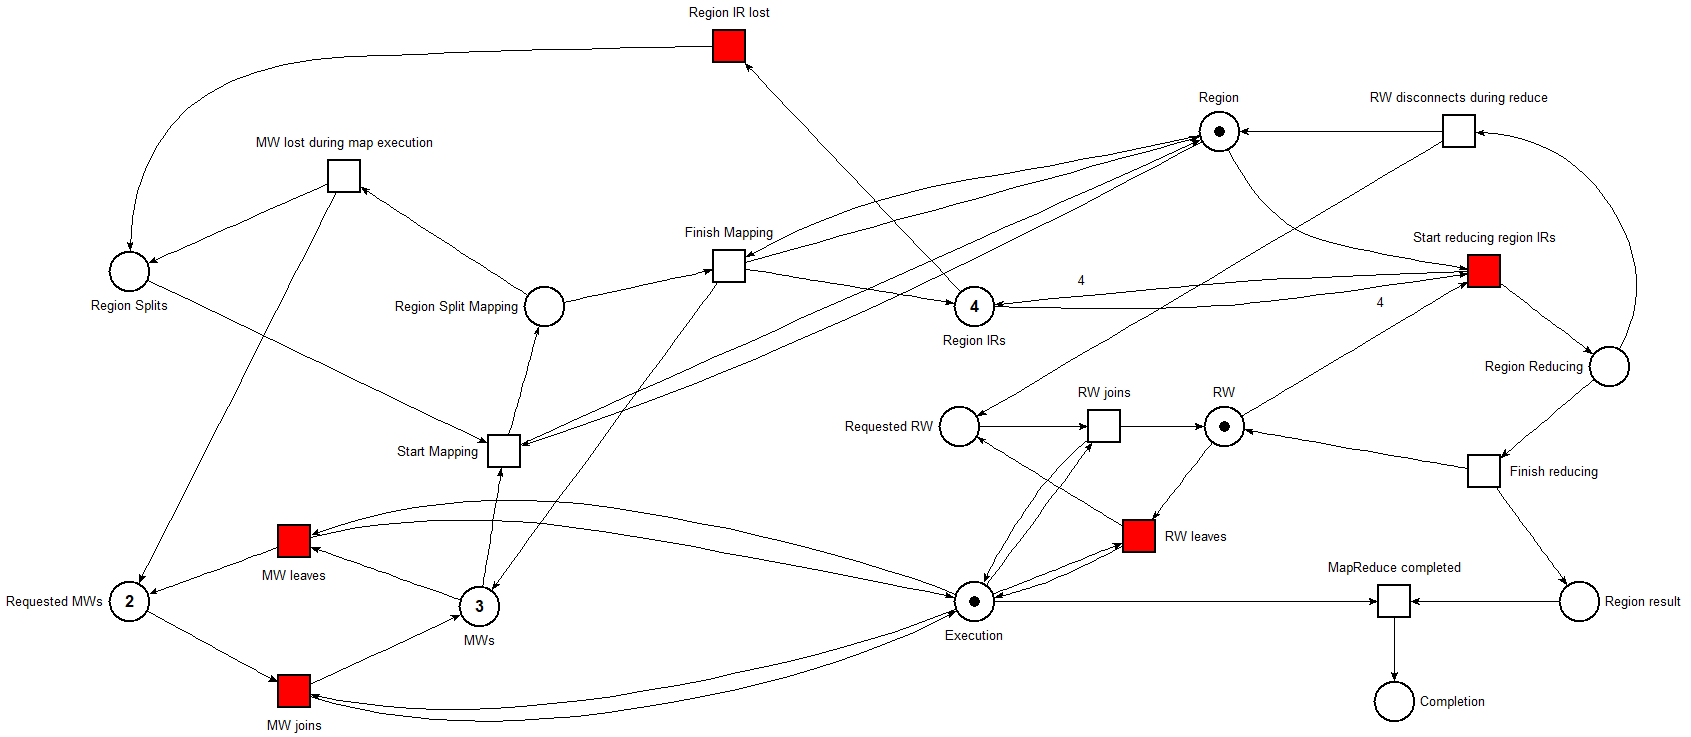
\includegraphics[width=\linewidth]{document/chapters/chapter_6/images/master_petri_net_3.png}
    \caption{MapReduce Master - Region Mapping completed}
    \label{fig:master_petri_net_3}
\end{figure}

\begin{figure}[!ht]
    \centering
    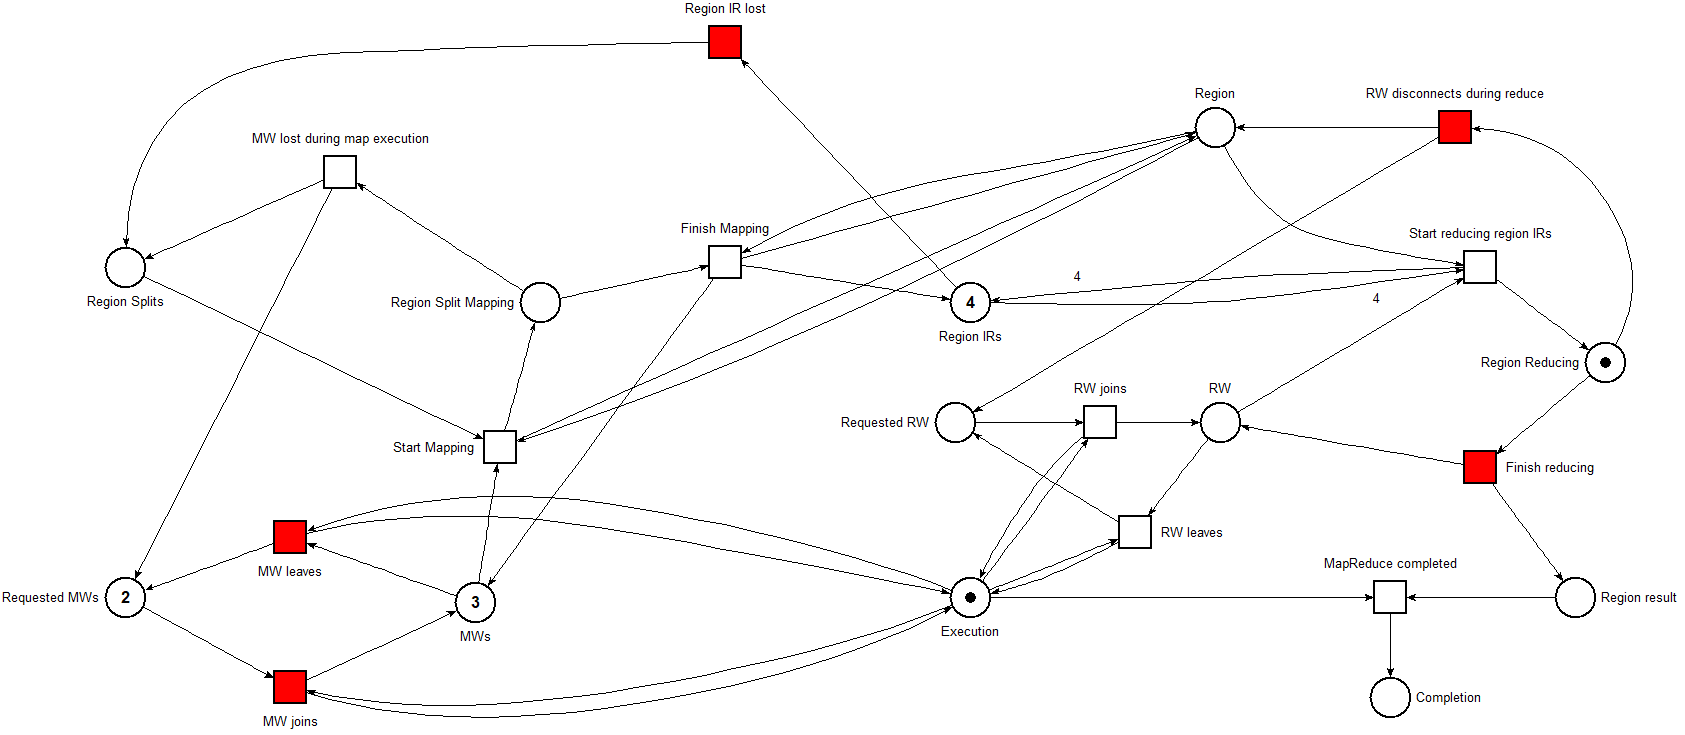
\includegraphics[width=\linewidth]{document/chapters/chapter_6/images/master_petri_net_4.png}
    \caption{MapReduce Master - Reducing process}
    \label{fig:master_petri_net_4}
\end{figure}

\begin{figure}[!ht]
    \centering
    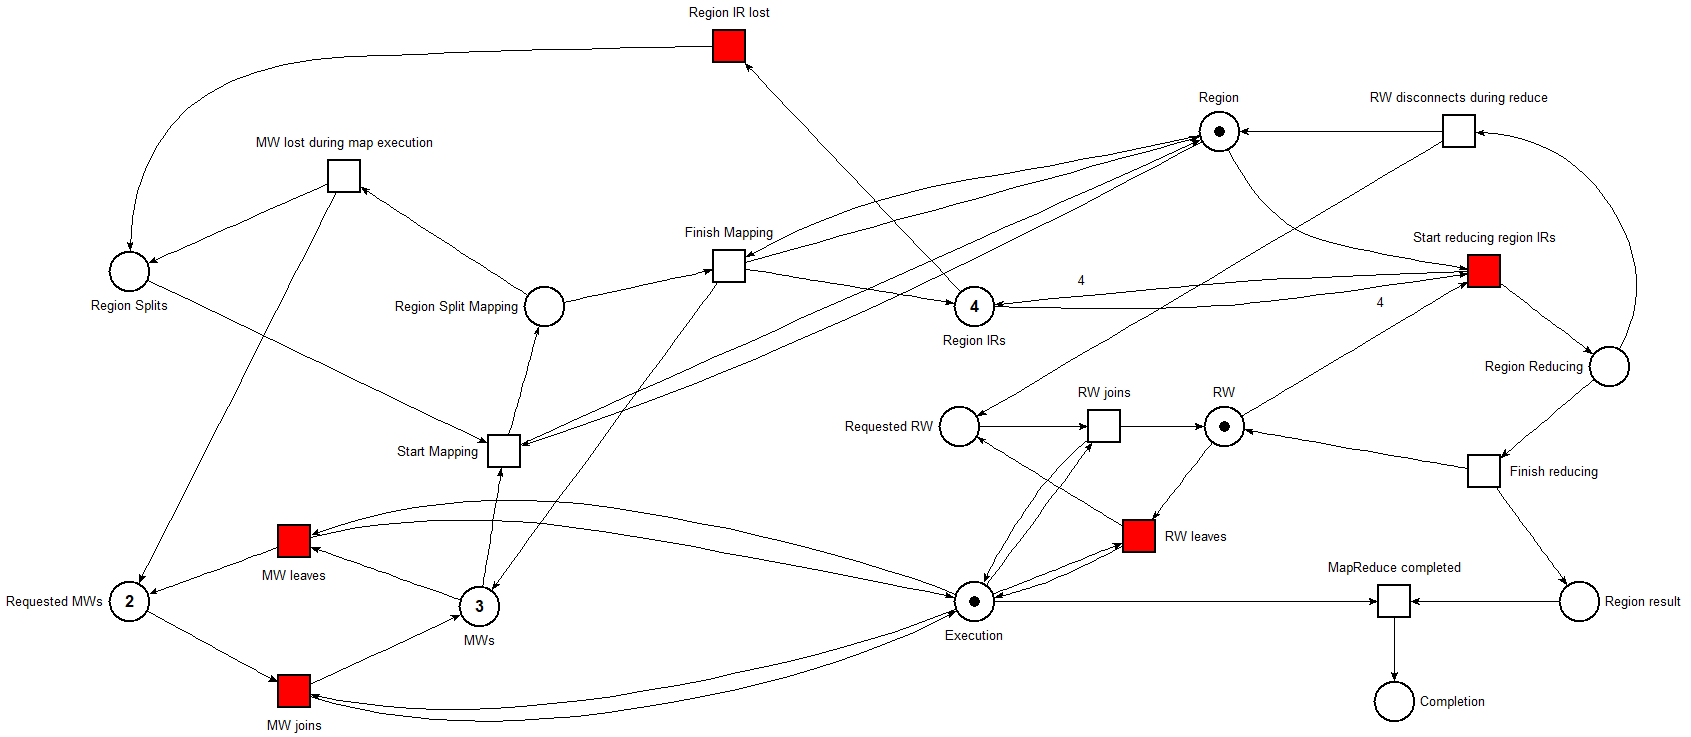
\includegraphics[width=\linewidth]{document/chapters/chapter_6/images/master_petri_net_5.png}
    \caption{MapReduce Master - Region completed}
    \label{fig:master_petri_net_5}
\end{figure}